\documentclass[pdftex,spanish]{pucthesis} 
\usepackage{graphicx}
\usepackage{float}
\usepackage{amsmath}
\usepackage{amsfonts}
\usepackage{amssymb}
\usepackage{times} % Fuente Times New Roman
\usepackage{booktabs}
\usepackage{hyperref}

% 1. Paquete para citas en formato APA
\usepackage[notocbib]{apacite}




\begin{document}

\mdate{Marzo, 2026}
\version{1}

\title[INFORME 2: RUTEO DE PROFESIONALES\\ GRUPO 10]
   {\bf INFORME 2: RUTEO DE PROFESIONALES DE LA SALUD\\ GRUPO 10}
\author[Integrantes:]{Integrantes:\\
\textnormal{\small{
Alonso Matta Sotomayor\\
Vicente Encalada Henríquez\\
Juan Andrés Muñoz Solano\\
Nicolás Provoste Moya\\
Benjamín Suazo Massaro}}
}

\address{Escuela de Ingenier\'ia\\
         Pontificia Universidad Cat\'olica de Chile\\ 
         Santiago, Chile}

\advisor{\textbf{Profesor Guía:} Steffan Widemann}
\ogrsmember{\textbf{Ayudante Tutor:} Fernanda Godoy}
\date{Marzo 2026}
\copyrightname{Grupo 10}
\copyrightyear{2026}

\NoChapterPageNumber
\pagenumbering{roman}
\maketitle

% --- ANEXOS Y DECLARACIÓN DE IA (OBLIGATORIO) [cite: 7151, 7161] ---
%\appendix
\chapter{Declaración de uso de IA}
\section*{Declaración de uso de IA en este informe y presentación asociada}

\textbf{Grupo:} 10 \\
\textbf{¿Hicieron uso de herramientas de IA?} SÍ

\textbf{Uso realizado:}
\begin{itemize}
    \item Apoyo a la redacción, ortografía y estructura gramatical.
    \item Búsqueda y filtro de literatura relevante al proyecto.
    \item Apoyo en el desarrollo de código computacional asociado al proyecto.
\end{itemize}

\textbf{Herramientas usadas:} Gemini (Google). \\
\textbf{Reflexión:} La herramienta fue un apoyo útil para estructurar la revisión bibliográfica inicial y organizar la sintaxis del código LaTeX, permitiendo un flujo de trabajo más eficiente.

\vspace{0.5cm}
\noindent \textbf{Integrantes y firmas:}

\vspace{0.5cm}

\begin{minipage}[t]{0.45\textwidth}
    \centering
    
\includegraphics[height=1.5cm]{figures/firma Alonso.jpeg} \\
    \rule{5cm}{0.4pt} \\
    Alonso Matta Sotomayor
\end{minipage}
\hfill
\begin{minipage}[t]{0.45\textwidth}
    \centering
    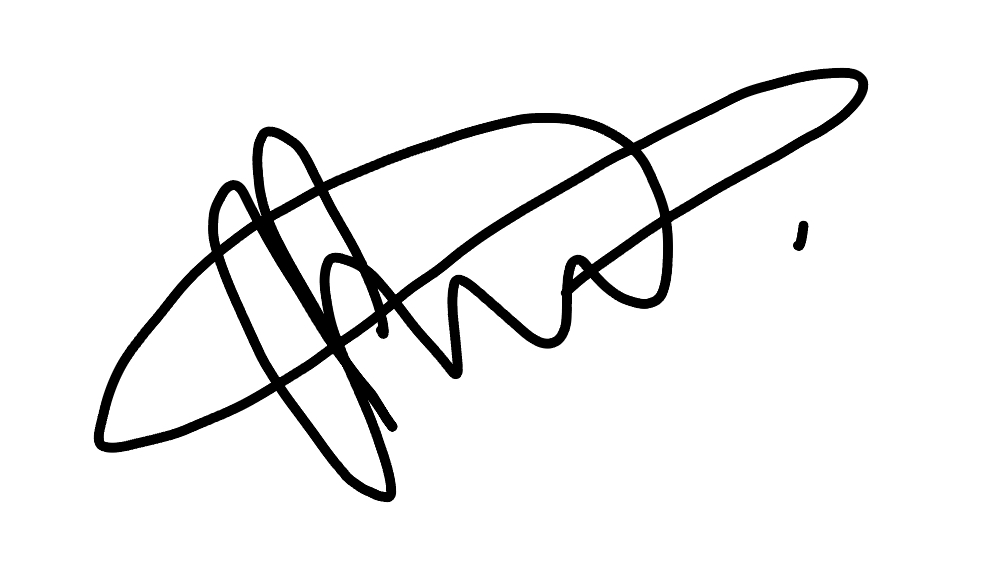
\includegraphics[height=1.5cm]{figures/IMG_1163.JPG} \\
    \rule{5cm}{0.4pt} \\
    Vicente Encalada Henríquez
\end{minipage}

\vspace{0.8cm}

\begin{minipage}[t]{0.45\textwidth}
    \centering
    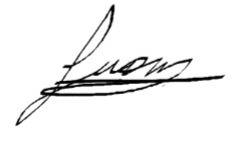
\includegraphics[height=1.5cm]{figures/firma juan muñoz.jpeg} \\
    \rule{5cm}{0.4pt} \\
    Juan Andrés Muñoz Solano
\end{minipage}
\hfill
\begin{minipage}[t]{0.45\textwidth}
    \centering
    
\includegraphics[height=1.5cm]{figures/firma Nico.jpeg} \\
    \rule{5cm}{0.4pt} \\
    Nicolás Provoste Moya
\end{minipage}

\vspace{0.8cm}

\begin{minipage}[t]{0.45\textwidth}
    \centering
    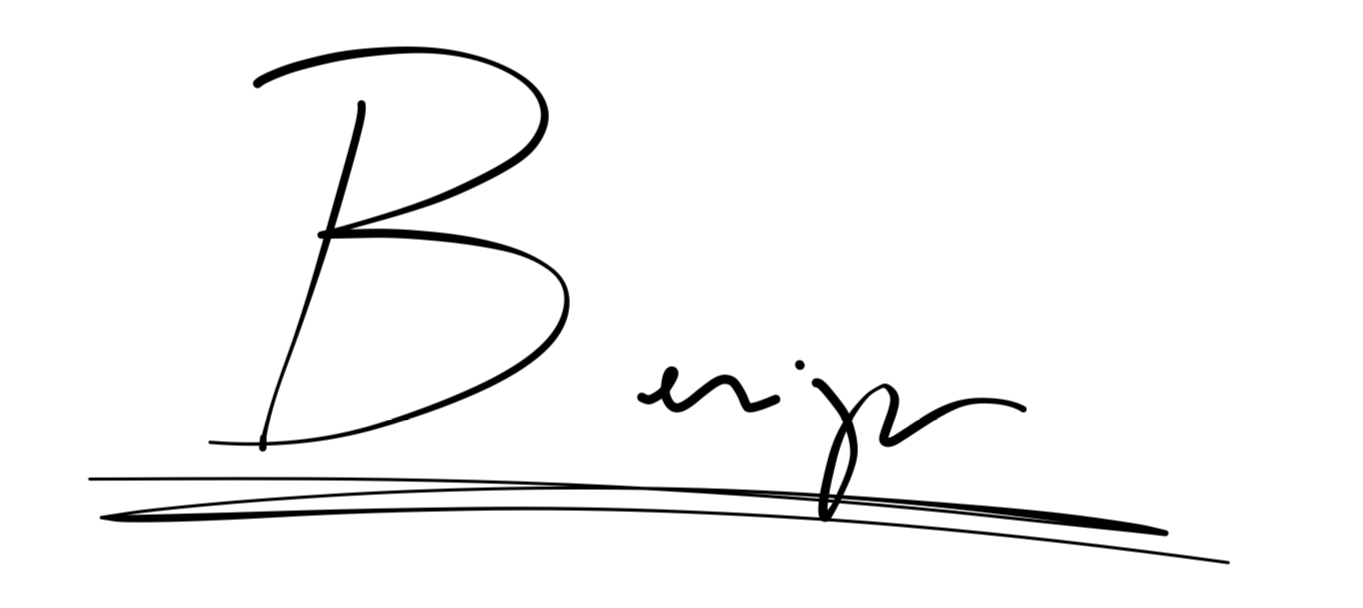
\includegraphics[height=1.5cm]{figures/firma benja.jpg} \\
    \rule{5cm}{0.4pt} \\
    Benjamín Suazo Massaro
\end{minipage}



% --- SECCIONES PRELIMINARES ---
\tableofcontents
%\listoffigures
\listoftables
\cleardoublepage


\phantomsection \label{resumen}
\chapter*{RESUMEN}
El presente proyecto aborda el desafío logístico de una empresa prestadora de servicios de salud en Santiago de Chile, centrada en la planificación diaria del transporte de más de 960 profesionales hacia y desde sus centros médicos. El problema se define técnicamente como un \textit{Time-Dependent Heterogeneous Dial-a-Ride Problem} (TD-HDARP), cuya complejidad radica en la integración de ventanas de tiempo estrictas, una flota de vehículos variada, y restricciones sindicales de compatibilidad entre pasajeros.

La metodología propuesta consiste en una arquitectura de solución híbrida: un modelo de \textit{Machine Learning (XGBoost)} para capturar la variabilidad del tráfico urbano, y la metaheurística \textit{Adaptive Large Neighborhood Search (ALNS)} para la optimización de rutas. El resultado final será un Sistema de Soporte a la Toma de Decisiones (DSS) desarrollado en Python, que automatiza la planificación y mejora indicadores clave como costos operacionales, ocupación de flota y puntualidad, en un máximo de una hora. El impacto del proyecto trasciende la eficiencia económica, asegurando la continuidad asistencial de los recintos de salud y mejorando el bienestar laboral de los profesionales al reducir su carga logística y mental.
\cleardoublepage



% --- CUERPO DEL INFORME (ESTRUCTURA SEGÚN LINEAMIENTOS) [cite: 7051, 7088] --- 
\chapter{Introducción} \label{ch:intro}
\section{Resumen del Caso de Estudio}

El caso se centra en el transporte diario (domicilio-trabajo o viceversa) de profesionales de la salud en turnos AM y PM en Santiago de Chile. El área de logística de la empresa de transporte debe diseñar rutas óptimas considerando los nodos origen--destino de cada profesional y sus horarios de turno.



%La organización busca planificar y optimizar el transporte diario de sus profesionales hacia y desde sus lugares de trabajo. Para lograrlo, el área de logística debe diseñar diariamente las rutas para distintos turnos, considerando las ubicaciones geográficas, las ventanas de tiempo requeridas y el estricto cumplimiento de normativas sindicales de comodidad.



%\section{Objetivos y complejidad del problema}
%El objetivo principal es desarrollar un modelo que genere rutas óptimas para minimizar los costos operacionales y la distancia recorrida. La complejidad radica en satisfacer restricciones sindicales de cuatro categorías de pasajeros, donde solo se permite transportar simultáneamente a personas de categorías consecutivas, además de cumplir con tiempos máximos de espera y viaje.







%Más allá del desafío puramente operacional de enrutar una flota y minimizar los costos de transporte , este problema reviste una profunda relevancia práctica para la estrategia de la empresa. El diseño de un sistema de transporte altamente confiable y puntual impacta de manera directa en el bienestar y la calidad de vida de los profesionales de la salud. Al disminuir la carga mental asociada al traslado diario y reducir significativamente las tasas de ausencias o retrasos, la empresa asegura la continuidad operativa de sus centros médicos, lo que se traduce de forma inmediata en una mejor calidad del servicio y atención entregada a los pacientes.

%Adicionalmente, resolver este problema logístico genera impactos corporativos tangibles. Por ejemplo, permite a la organización fortalecer su reputación institucional, retener talento al ofrecer mejores condiciones laborales y consolidar su posición en el mercado de la salud. Por último, la optimización eficiente de los vehículos compartidos alinea a la empresa con metas de sostenibilidad y responsabilidad social, reduciendo la huella de carbono de sus operaciones y mitigando su impacto en la congestión vehicular urbana.










%\section{Objetivos y Complejidad del Problema}

%El objetivo es desarrollar un modelo que genere rutas óptimas minimizando costos operacionales, definidos por tipo/cantidad de vehículos a utilizar y su distancia recorrida. El problema exige respetar estrictas restricciones temporales y sindicales, incluyendo tiempos máximos de espera y compatibilidad entre categorías de pasajeros.



\section{Relevancia Práctica e Impacto Real}

La resolución de este problema logístico trasciende la optimización matemática de rutas. Representa una decisión estratégica que fortalece directamente la propuesta de valor y competitividad de la empresa a través de tres dimensiones fundamentales:

%POSIBLE RESUMEN DE LO ANTERIOR POR TEMAS DE ESPACIO
%la \textbf{continuidad operativa}, asegurando que el personal crítico llegue puntualmente a sus turnos; el \textbf{bienestar laboral}, al transformar el transporte en un beneficio que reduce el estrés del personal médico; y la \textbf{eficiencia corporativa}, optimizando el uso de recursos y disminuyendo costos operacionales.



\begin{itemize}
    \item \textbf{Continuidad operativa y calidad asistencial:} En el sector de la salud, la puntualidad del personal es un factor crítico. Un sistema de transporte confiable mitiga directamente los riesgos asociados a ausencias o retrasos. Al garantizar que los profesionales lleguen a sus turnos de manera oportuna, la empresa asegura la continuidad de sus operaciones y, en consecuencia, mantiene un alto estándar en la calidad del servicio entregado a los pacientes.
    
    \item \textbf{Bienestar laboral y retención de talento:} El cumplimiento riguroso de las normativas sindicales respecto a los tiempos de viaje no es solo una restricción del modelo, sino una herramienta de cuidado al trabajador. Optimizar el traslado disminuye significativamente la carga mental y el estrés de los profesionales de la salud. Esto se traduce en un mejor clima laboral, fortaleciendo la reputación institucional y posicionando a la empresa como un lugar atractivo para retener talento clave.
    
    \item \textbf{Sostenibilidad y eficiencia corporativa:} Desde una perspectiva organizacional, consolidar los viajes compartidos de manera eficiente permite cuidar el presupuesto al reducir costos operacionales innecesarios. Paralelamente, esta eficiencia alinea a la empresa con sus objetivos de responsabilidad social y ambiental, ya que una menor cantidad de vehículos en tránsito contribuye activamente a la reducción de la huella de carbono y alivia la congestión del tráfico urbano en Santiago.
\end{itemize}


\section{Propuesta}
Para materializar este valor, se propone el desarrollo de un \textbf{Sistema de Soporte a la Toma de Decisiones (DSS)} programado en Python. Esta herramienta operará como un \textit{pipeline integral} que procesará automáticamente las solicitudes de viaje, incorporando un modelo predictivo de tráfico y una metaheurística de ruteo (ALNS) para generar hojas de ruta óptimas en una hora o menos. Con esto, se ofrece una solución técnica que automatiza y profesionaliza la planificación diaria de la flota.



%Se propone una metodología que permita ejecutar el modelo para que los viajes compartidos sean competitivos y eficientes, optimizando rutas y la asignación de clientes, cumpliendo con las restricciones y objetivos planteados, clasificando el caso como un problema relevante de optimización de rutas de transporte de personal.

%Para materializar aquello, el entregable final consistirá en un Sistema de Soporte a la Toma de Decisiones (DSS) desarrollado en Python. Este leerá y procesará las solicitudes de viajes e integrará el modelo predictivo de tráfico con una metaheurística de enrutamiento para procesar las restricciones en un tiempo límite de una hora, generando automáticamente hojas de ruta detalladas para los despachadores de la flota. De esta forma, se ofrece una solución integral que automatiza y optimiza la planificación diaria del transporte.

\chapter{Descripción detallada del problema} \label{ch:problema}
A continuación, se describe el problema y el caso de estudio, junto con un análisis teórico y de datos asociados, y el abordaje profundo de los objetivos y las motivaciones.

\section{Descripción del Problema}

El caso, en primera instancia representa un problema de enrutamiento logístico. Durante la mañana de una jornada laboral, cada profesional de la salud se inscribe solicitando transporte para el día siguiente, ya sea para el turno AM (ruta domicilio-trabajo) o PM (ruta trabajo-domicilio), indicando sus horarios disponibles. Las rutas se planifican durante la tarde del día de la inscripción.

El problema se debe abordar con el fin de minimizar los costos operacionales, mediante cuatro decisiones clave: selección de flota (cantidad y tipo de vehículo a despachar), asignación de pasajeros (respetando compatibilidades sindicales), secuenciación de rutas (orden geográfico de paradas) y programación horaria (tiempos exactos de recogida y entrega sin exceder límites de espera o viaje).

El modelo considera los recursos de la empresa, que dispone de una flota de vehículos variada en términos de tipo y espacio. El uso de un vehículo tiene asociado un costo fijo, el cual se cobra independientemente de la cantidad de personas dentro de este (es decir, estando vacío, incompleto o lleno, el cobro se realiza de todas formas), y un costo variable por kilómetro recorrido. 

Existen, además, las restricciones de cumplimiento obligatorio, que si bien no hay penalizaciones por incumplimiento, este no puede ocurrir:
\begin{itemize}
    \item Categorías de pasajeros: cuatro grupos, con transporte simultáneo permitido solo entre dos categorías consecutivas (ej. 1 y 2, o 3 y 4).
    \item Restricciones temporales: los profesionales no pueden llegar demasiado temprano ni permanecer excesivo tiempo en el vehículo.
    \item Viaje individual: permitido si el trayecto directo hogar-trabajo supera el límite máximo de tiempo.
\end{itemize}

Además del desafío de optimización combinatoria, el problema presenta una segunda vertiente fundamental de carácter predictivo. Según los antecedentes históricos de la empresa, existe una discrepancia demostrada entre los tiempos de viaje pronosticados por los proveedores de ruteo estándar y los tiempos de viaje reales observados en terreno. 

Dado que las ventanas de tiempo son sumamente estrictas (con márgenes de hasta solo 5 minutos para ciertas prioridades), planificar las rutas basándose en estimaciones teóricas erróneas conllevaría inevitablemente a retrasos operativos y a la violación de las normativas sindicales. Por lo tanto, la segunda parte del problema exige analizar la información histórica de la flota para crear un mecanismo de ajuste de tiempos, evaluando aspectos como la puntualidad. El modelo final no solo debe "rutear", sino que debe garantizar que las hojas de ruta generadas sean precisas, ejecutables en la realidad y robustas ante las variaciones del tráfico.






\section{El Problema en la Literatura}

Según la descripción y una exhaustiva revisión bibliográfica, el problema se clasifica como un \textit{Time-Dependent Heterogeneous Dial-a-Ride Problem} (de ahora en adelante TD-HDARP) \cite{Ho2018, Parragh2011}.

Un problema de transporte a demanda dependiente del tiempo (parte TD-DARP de la abreviatura) nace de solicitudes de transporte con ubicaciones de recogida y entrega, número de pasajeros, ventanas de tiempo y límites máximos de viaje, en el cual se debe optimizar rutas y asignación de pasajeros \cite{Gaul2025}. Esta última frase, simplifica de forma correcta y precisa lo que se desea abordar en el caso de estudio.

Los problemas de ruteo cada vez se vuelven más complejos debido a la demanda creciente de transporte y el aumento en la cantidad de flota de vehículos \cite{Gaul2025}. Por ello y según la información otorgada, considerar dentro del caso de estudio una flota heterogénea (H de la abreviatura), permite evaluar la complejidad del uso de las distintas capacidades según el tipo de vehículo que posee la empresa.

Por otro lado, los problemas tipo DARP suelen ser clasificados como \textit{Non-deterministic Polynomial-time hard} (NP-Hard), una clase de optimización combinatoria, la cual tiene tiempos de cálculo que crecen exponencialmente \cite{TaylorFrancisNPHard}. En otras palabras, aunque existen métodos exactos que garantizan la solución óptima, el tiempo computacional requerido para resolver instancias de tamaño real crece exponencialmente, volviéndolos inoperantes para la toma de decisiones diarias \cite{Izadkhah2022}.




\section{Objetivo y Motivación}
El objetivo central es desarrollar un modelo matemático que capture fielmente las complejidades del problema, logrando un equilibrio entre la minimización de costos operativos y la satisfacción de las restricciones.

La motivación de este trabajo reside en aplicar la investigación operativa para impactar directamente el ámbito de la salud. Al optimizar la movilidad, se busca mitigar el estrés de los profesionales y potenciar su eficiencia operativa, mejorando su bienestar integral. Asimismo, en el marco de los problemas DARP, estas soluciones son fundamentales para un futuro sostenible al reducir la congestión y las emisiones contaminantes, mitigando así el impacto ambiental negativo \cite{Gaul2025}.


\section{Análisis de los Datos} %considerar mover las tablas a los anexos en caso de que falte espacio

Los datos proporcionados se clasifican en tres grandes categorías: instancias operativas (archivos con extensión xlsx), matrices de tiempo y distancias (archivos con extensión csv con prefijo "times") y una muestra de tiempos reales observados. Todas las tablas que se mencionen para el análisis se encuentran en la sección Anexos.

\subsection{Instancias Operativas}

En Tabla \ref{tab:instancias operativas}, es posible observar que en la instancia AM, los 620 profesionales deben ser recogidos en sus domicilios y entregados a su lugar de trabajo. La hora más temprana de recogida (Pickup From) varía entre las 04:15 y las 06:00, mientras que el inicio de turno (Turn Start) se extiende desde las 04:35 hasta las 06:45. Las franjas de mayor concentración son las 04:50 (226 profesionales) y las 04:40 (110 profesionales). La ventana de tiempo promedio disponible entre la hora de recogida más temprana y el inicio del turno es de 42.6 minutos (con una desviación de 11.3 minutos) con un mínimo de solo 5 minutos y un máximo de 72 minutos.

En la instancia PM, los 347 profesionales de la salud deben ser recogidos desde su lugar de trabajo a sus domicilios. La hora de fin de turno (Turn End) se distribuye principalmente en dos bloques: uno cercano a la medianoche (68 pasajeros a las 00:11, junto a otros horarios entre las 00:00 y las 00:06) y otro entre las 22:46 y las 23:56 donde se posicionan la mayoría de los profesionales. Los horarios más frecuentes son las 23:01 (79 profesionales) y las 00:11 (68 profesionales).

Ambas instancias se clasifican además a los profesionales en 4 niveles de prioridad, tal y como se observa en Tabla \ref{tab:distribucion por prioridad}. La mayoría de los profesionales se concentra en las prioridades 2 y 3, representando conjuntamente más del 75\% en ambas instancias. La prioridad 4 es marginal (menor al 6\%), lo cual es relevante para el modelo dado que sus restricciones sindicales son más exigentes. 

Cabe mencionar que las restricciones sindicales son idénticas para ambas instancias. Un detalle clave tras analizar estos datos, que se evidencia en Tabla \ref{tab:tiempos de espera y en vehi} es que la restricción de tiempo de espera más crítica es la de prioridad 4, solos 5 minutos de espera y 50 minutos como tiempo máximo en vehículo, esto limita fuertemente la posiblidad de agrupar esta prioridad con otra.

También se dispone de dos tipos de vehículos, la cantidad y precio respectivo a estos se puede encontrar en Tabla \ref{tab:flota de vehi}. El costo variable por distancia es de 800 CLP/km para ambos tipos. Los tiempos de parada son de 3 minutos para recogida (pickup) y 1 minuto para entrega (delivery).

Finalmente se tiene el factor geográfico, donde los puntos de recogida en la instancia AM abarcan una amplia zona de Santiago, con latitudes entre -33,75 y -33,18 y longitudes entre -70,89 y -70,52. Los centros de trabajo presentan una dispersión menor (latitud entre -33,61 y -33,37; longitud entre -70,76 y -70,53), sugiriendo que los centros médicos están relativamente concentrados en comparación con los domicilios de los profesionales. La instancia PM muestra un patrón invertido coherente con la instancia AM.

\subsection{Matrices de Tiempo y Distancia}

Se proporcionan 7 archivos CSV con tiempos y distancias pronosticados entre todos los pares de nodos (origen-destino) para horas específicas. Cada matriz posee 409.600 pares para AM y 134.689 para PM.

Un hallazgo interesante es la variación de tiempos de viaje según la hora, evidenciando la naturaleza de dependencia temporal del problema (Tabla \ref{tab:var de tiempos}). En la jornada AM, los tiempos aumentan conforme avanza la mañana. En la jornada PM, la hora 22:00 presenta los tiempos más altos (28.6 min en promedio de viaje y velocidad de 33.9 km/h), siendo aproximadamente un 15\% más lenta que las horas de la madrugada. Las distancias se mantienen prácticamente constantes entre las diferentes horas (media de aproximadamente 16.6 km en instancia AM y 16.6 km en instancia PM), esto permite inferir que las variaciones con respecto a la media se pueden explicar por fluctuaciones en el tráfico y no a cambios en la ruta del proveedor del servicio. Estos viajes consideran todas las combinaciones posibles (domicilio/centro de trabajo, domicilio/domicilio, centro de trabajo/centro de trabajo y centro de trabajo/domicilio).



\subsection{Muestras de Tiempos Reales}

El archivo entregado para esta sección contiene 15.000 observaciones de viajes reales, recopiladas entre el 1 y el 14 de marzo del 2026. Para cada viaje se registran las coordenadas de origen y destino, la fecha/hora de partida, el tiempo pronosticado por el proveedor y el tiempo real observado.

El análisis de esta muestra es la pieza central para resolver la segunda parte del problema: el ajuste de tiempos. Al observar la Tabla \ref{tab:comparativa}, se evidencia empíricamente la discrepancia entre la teoría y la realidad (por ejemplo, tiempos reales que alcanzan los 5.881 segundos frente a pronósticos que estimaban la mitad). Estas diferencias indican que no es factible utilizar los tiempos del proveedor de forma directa. Por ende, estos datos históricos servirán como conjunto de entrenamiento para desarrollar un modelo predictivo capaz de capturar estos márgenes de error y ajustar la matriz de tiempos del enrutador, garantizando que la planificación de las rutas sea fiel a las condiciones reales de operación.

\subsection{Caracterización de la Demanda y Concentración Temporal}

El análisis de las instancias revela una asimetría en la carga de trabajo entre jornadas, con 620 profesionales para el turno AM y 347 para el PM. En la mañana, se observa una densidad crítica de demanda: el 36\% de los profesionales (226 personas) requiere ser recogido a las 04:50, lo que genera un pico operativo en un intervalo de tiempo muy reducido. Asimismo, aunque la ventana de tiempo promedio para el traslado es de 42.6 minutos, existen casos críticos con solo 5 minutos de holgura, lo que elimina cualquier margen de error ante contingencias viales.

\subsection{Impacto en las Restricciones Sindicales en la Eficiencia}

El análisis de la distribución por prioridad revela un condicionante crítico para la optimización de las rutas. Según los datos recopilados, más del 75\% de los profesionales se concentran en las prioridades 2 y 3. No obstante, la categoría 4, aunque representa menos del 6\% de la demanda total, actúa como el principal limitador de la eficiencia operativa debido a sus estrictas restricciones sindicales: solo 5 minutos de tiempo máximo de espera y un límite de 50 minutos de permanencia en el vehículo.

Dado que un vehículo solo puede transportar simultáneamente a pasajeros de a lo más dos categorías distintas y estas deben ser consecutivas, la baja densidad de pasajeros de prioridad 4 reduce drásticamente las probabilidades de consolidar esta prioridad con la 3. Esta posible fragmentación del espacio de soluciones factibles sugiere que el modelo podría converger a una tendencia de generar viajes de baja ocupación o trayectos casi directos para esta categoría, elevando el costo marginal por pasajero y dificultando el aprovechamiento total de la capacidad de la flota.

\subsection{Outliers y Limpieza de Datos}
A partir de la Tabla \ref{tab:comparativa}, existen:
\begin{itemize}
    \item \textbf{Valores atípicos superiores:} Se registran tiempos reales de hasta 5.881 segundos, superando con creces el máximo pronosticado de 3.250 segundos. Estos registros representan eventos de congestión extrema que podrían inducir a que un posible algortimo de aprendizaje automático sufra de error.
    
    \item \textbf{Inconsistencias de duración mínima:} El registro de viajes reales de solo 6 segundos para distancias que promedian los 16.6 km sugiere ruido o errores de captura en el sistema de telemetría, por lo que dentro de los próximos pasos se buscará verificar el volumen de datos por deciles y ver la dispersión entre los datos, para determinar posibles outliers y descartarlos en la medida que aporten más ruido a los datos.
\end{itemize}




\section{Indicadores de Desempeño (KPI's)}
Para evaluar la calidad del modelo a implementar y contrastarlo con una línea base, se definen cuatro indicadores clave de desempeño. 

\begin{itemize}
    \item \textbf{Costo operacional total:} Gasto total de los viajes. Suma el cobro base de cada vehículo (2.200 pesos para el normal y 4.500 pesos para el grande) más los 800 pesos que cuesta cada kilómetro recorrido. Esto nos dice directamente si estamos cuidando el presupuesto de la empresa.
    \item \textbf{Distancia total recorrida:}
    Mide los kilómetros acumulados por la totalidad de la flota en operación durante una jornada. Este indicador refleja la eficiencia en la configuración de la ruta, permitiendo validar si el orden de los puntos de encuentro y llegada optimiza el trayecto geográfico.
    \item \textbf{Tasa de ocupación de flota:} Cuantifica la eficiencia en el uso de las capacidades de los vehículos utilizados, considerando que un tipo de vehículo posee 3 asientos y el otro 6 asientos. Es un indicador de gran importancia debido a su relación con la complejidad de la restricción sindical. Una tasa de ocupación alta demuestra la robustez del algoritmo para consolidar a profesionales compatibles de manera inteligente, maximizando el aprovechamiento de la flota sin comprometer las restricciones de comodidad.
    \item \textbf{Tiempo promedio de permanencia y espera:}
    Monitorea el tiempo transcurrido desde el abordaje hasta la llegada a su destino. Minimizar este promedio es muy importante para garantizar el bienestar laboral.

\end{itemize}

Cada uno de los KPI's mencionados permitiran medir no solo la eficiencia económica del sistema, sino también el nivel de servicio y el cumplimiento de los objetivos estratégicos de la empresa.



\chapter{Discusión metodológica} \label{ch:metodologia}
En este capítulo se analizan en profundidad las metodologías identificadas en la literatura científica para resolver el problema de ruteo de profesionales de la salud, clasificado como un TD-HDARP. Dado que es un problema de complejidad NP-Hard, se debe evaluar el equilibrio entre la calidad de la solución obtenida y el tiempo de cómputo requerido para su ejecución \cite{Cordeau2003}. Sobre la base del análisis cualitativo se construye una formalización matemática completa del problema, una estrategia de Caso Base defendible y una especificación algorítmica del ALNS adaptada de la evidencia reciente en contextos análogos.

\section{Análisis de Metodologías Atingentes}

A continuación, se presentan las tres grandes familias de métodos de resolución identificadas para este caso de estudio, contrastando sus características frente a las necesidades del proyecto y los datos históricos disponibles.

\subsection{Métodos Exactos: Programación Lineal Entera Mixta (MILP)}
Estos métodos buscan encontrar el óptimo global mediante algoritmos como \textit{Branch-and-Cut} o la Generación de Columnas (\textit{Branch-and-Price}) utilizando solucionadores como Gurobi \cite{Cordeau2006}. Si bien estos enfoques poseen la ventaja de garantizar la obtención matemática del óptimo global y de proveer cotas inferiores, sufren cuando se enfrentan a problemas de alta dimensionalidad. La evidencia científica señala que algoritmos exactos rara vez logran resolver a optimalidad instancias de DARP que superen las cincuenta solicitudes de transporte en tiempos computacionales razonables. Considerando que la instancia AM del caso de estudio requiere consolidar la demanda de 620 pasajeros, la excesiva demora de los métodos exactos los vuelve operativamente inviables para este caso. No obstante, la formalización MILP es imprescindible como referencia teórica y como oráculo sobre instancias reducidas (Caso Base).

\subsection{Generación de Solución Inicial: Heurísticas Constructivas}
Dado que las metaheurísticas (como ALNS) son algoritmos de mejoramiento, requieren obligatoriamente de una solución inicial sobre la cual iterar. En la literatura existen dos enfoques clásicos: la Heurística de Inserción Paralela con Ventanas de Tiempo \cite{Jaw1986} y variantes secuenciales de inserción aleatoria en múltiples rutas \cite{Pilati2025}. La primera garantiza factibilidad inicial pero impone un sesgo geométrico que puede restringir la exploración posterior; la segunda admite soluciones iniciales infactibles que el ALNS corrige mediante penalizaciones dinámicas, ofreciendo mayor diversidad. Para este proyecto se adopta el enfoque de \cite{Pilati2025}, por su compatibilidad directa con el mecanismo adaptativo del ALNS seleccionado y porque su implementación es computacionalmente más liviana.

\subsection{Metaheurísticas: Tabu Search vs. ALNS}
Para la fase de optimización, se evaluaron dos metaheurísticas predominantes: la Búsqueda Tabú (\textit{Tabu Search}) y \textit{Adaptive Large Neighborhood Search} (ALNS).

Es importante aclarar que las limitaciones de \textit{Tabu Search} no son inherentes a su marco teórico, sino a la naturaleza de los operadores clásicos de búsqueda local que suele emplear (como \textit{Swap} o \textit{Relocate}). En un problema con restricciones sindicales estrictas y límites de tiempo críticos, el espacio de soluciones factibles está altamente fragmentado. Un operador de \textit{Tabu Search} tradicional generaría vecindarios donde la gran mayoría de los movimientos resultan infactibles, limitando severamente la exploración.

En contraste, ALNS aborda este problema mediante la destrucción y reconstrucción a gran escala \cite{Ropke2006}. Al remover una fracción significativa de las solicitudes en una sola iteración, ALNS es capaz de ``saltar'' las barreras de infactibilidad geométrica y temporal, alcanzando regiones del espacio de búsqueda inalcanzables para búsquedas locales tradicionales. Adicionalmente, la adaptabilidad de los pesos de sus operadores permite al algoritmo auto-calibrarse al problema específico, sin requerir ajuste manual caso a caso.

Por este motivo, se selecciona ALNS de manera definitiva. Los operadores específicos, la función de evaluación con penalizaciones dinámicas y el criterio de aceptación se especifican formalmente en la Sección~\ref{sec:alns}.

\subsection{Otras Alternativas}
Otras metaheurísticas ampliamente utilizadas en DARP y variantes similes como el VRP también fueron revisadas, con el objetivo de evaluar alternativas adicionales a ALNS. Sus consideraciones fueron en función de las restricciones del proyecto, analizando su capacidad de respuesta ante cada una de ellas.

\begin{itemize}
    \item \textbf{Variable Neighborhood Search (VNS)}
\end{itemize}

VNS ha mostrado buen desempeño en VRPTW y HFVRP \cite{Hansen2010}, y ha sido aplicado a DARP por Parragh (2011). Sin embargo, a partir de este último es posible inferir que sus vecindarios incrementales tienden a generar tasas muy altas de invianilidad al no respetar restricciones de compatibilidad ni considerar ventanas de tiempo rígidas, lo cual reduce su eficiencia exploratoria en problemas “ricos” como TD-HDARP.

\begin{itemize}
    \item \textbf{Iterated Local Search (ILS)}
\end{itemize}

También se encuentra ILS, la cual es una metaheurística competitiva en VRP clásico \cite{Lourenco2003}, pero los experimentos asociados y su razonamiento teórico reflejan una fuerte dependencia en la calidad de la solución inicial. En problemas con espacio factible fragmentado, como ocurre con tiempos máximos en vehículo y límites sindicales del DARP asociado a este proyecto, tiende a quedar atrapada en atractores locales.

\begin{itemize}
    \item \textbf{Hybrid Genetic Algorithm (HGA) \cite{Sohrabi2024}}
\end{itemize}
Finalmente, se considera la metaheurística híbrida (HGA), la investigación de Sohrabi et al. (2024) demuestran que permite explorar un espacio de búsqueda más amplio gracias al uso de poblaciones y operadores evolutivos, maneja bien soluciones infactibles sin necesidad de penalizaciones e incorpora diversidad adaptativa, presentando resultados competitivos incluso DARP con flotas heterogéneas. Dentro de sus desventajas se encuentra que requiere calibrar parámetros evolutivos como el tamaño poblacional y puede ser menos interpretable operacionalmente que heurísticas clásicas como VNS. Sin embargo, el mayor problema nace de las restricciones adicionales de este proyecto como la compatibilidad entre categorías y viajes bidireccionales, donde el HGA está diseñado para restricciones continuas y no categóricas duras. La integración de estas impiden que se generen los buenos resultados presentados por Sohrabi, descartando finalmente su uso.

En contraste de estas últimas alternativas consideradas, ALNS ha demostrado consistentemente un desempeño superior en variantes “ricas” del DARP. Su diferencia crítica es que la arquitectura modular de ALNS permite incorporar restricciones duras mediante operadores de reparación específicos. En este proyecto, reglas sindicales y compatibilidades categóricas se integran directamente en los operadores de inserción y en el verificador de factibilidad, garantizando que el algoritmo nunca genere rutas que violen estas restricciones. Esta capacidad de “personalización de operadores” es una ventaja que no poseen ni VNS, ni ILS ni HGA, cuyos movimientos o cruces pueden generar configuraciones irrecuperables bajo dichas reglas. Por tanto, ALNS presenta el mejor equilibrio entre flexibilidad, calidad de solución, cumplimiento de restricciones y tiempo computacional para el problema estudiado.



\subsection{Integración de Tiempos Dependientes (TD) y Modelos Predictivos}
El componente \textit{Time-Dependent} (TD) del problema exige que la función objetivo incorpore tiempos de viaje $\tau_{ij}(t)$ que no son estáticos, sino que dependen directamente de la hora de inicio del viaje $t$. Como se evidenció en el análisis de datos empíricos del Capítulo~\ref{ch:problema}, los tiempos de viaje fluctúan según el horario.

Para alimentar al algoritmo ALNS con una matriz de tiempos dinámica, se empleará un modelo predictivo basado en XGBoost (\textit{Extreme Gradient Boosting}) \cite{Chen2016}. Este modelo de aprendizaje automático es apto para capturar las relaciones no lineales del tráfico en Santiago utilizando los datos históricos entregados, entrenado minimizando el error cuadrático medio (MSE) entre el tiempo pronosticado y el real, calibrando hiperparámetros tales como \texttt{n\_estimators}, \texttt{max\_depth} y \texttt{learning\_rate}.

Esta hibridación entre modelos predictivos (XGBoost para calcular $\tau_{ij}(t)$) y prescriptivos (ALNS para optimizar la asignación) es la propuesta central para abordar la complejidad del TD-HDARP.

\section{Aplicación de ALNS en Contextos Análogos}
\label{sec:papers}

Además del marco teórico original de \cite{Ropke2006}, se revisan tres trabajos recientes que aplican ALNS a variantes del DARP en contextos cercanos al presente: \cite{Pilati2025} aporta el esqueleto de la función de evaluación con penalizaciones dinámicas, mientras que \cite{Zhao2022} y \cite{Portell2024} fundamentan el tratamiento del time-dependency y la integración de modelos predictivos.

\subsection{Pilati et al. (2025): Transporte de Pacientes Dependientes}
\cite{Pilati2025} resuelven un DARP estático con flota homogénea y depósito único para la Austrian Red Cross, minimizando el tiempo total de viaje bajo ventanas de tiempo, tiempos máximos de viaje y jornadas fijas. La principal contribución que adoptamos es su \textbf{función de evaluación con penalizaciones dinámicas},
\begin{equation}
\label{eq:eval-pilati}
f(s) = c(s) + \alpha\, q(s) + \beta\, r(s) + \gamma\, d(s) + \varepsilon\, t(s),
\end{equation}
donde $q, r, d, t$ son violaciones de carga, tiempo en vehículo, jornada y ventanas, y los pesos se multiplican (o dividen) por $\delta\sim U(0{,}05,0{,}10)$ según si la restricción se viola o no. Solo soluciones con $f(s)=c(s)$ (estrictamente factibles) pueden ser incumbentes, permitiendo explorar transitoriamente regiones infactibles sin abandonar la dirección hacia el óptimo. Su implementación, validada sobre el \textit{benchmark} de \cite{Parragh2011}, obtiene soluciones a lo más $5\%$ peores en 18 de 20 instancias. Nuestra variante extiende el esquema incorporando flota heterogénea, tiempos dependientes $\tau_{ij}(t)$ y restricciones sindicales categóricas; por ello agregamos un término $\phi\,u(s)$ a \eqref{eq:eval-pilati} (ver Sección~\ref{sec:alns}).

\subsection{Zhao et al. (2022) y Portell \& Lourenço (2024): Tratamiento del TD}
Dos trabajos recientes validan, desde ángulos complementarios, el manejo de $\tau_{ij}(t)$ en DARP sanitarios. \cite{Zhao2022} estudian un TD-PDARP \textit{single-vehicle} para ambulancias no-emergencia de la Hong Kong Hospital Authority y proponen un procedimiento de evaluación de factibilidad bajo tiempos dependientes de la hora de partida que justifica nuestras matrices horarias escalonadas y la fase de búsqueda local intra-ruta tras cada movimiento destroy--repair (su híbrido ALNS+LS obtiene el óptimo en el $1{,}03\%$ del tiempo de Gurobi). Por su parte, \cite{Portell2024} abordan un DARP heterogéneo ``rico'' (rHDARP) para el transporte de personas con movilidad reducida en Barcelona, integrando flota mixta (taxis y buses adaptados), múltiples depósitos y un modelo predictivo de \textit{machine learning} para estimar $\tau_{ij}(t)$ según hora y día. Es la referencia más cercana al presente caso pues valida simultáneamente los tres ejes que combinamos aquí (heterogeneidad de flota, dependencia temporal y predicción ML); adoptamos explícitamente su arquitectura en dos capas (predictiva con XGBoost, prescriptiva con ALNS/MILP), omitiendo el multi-depósito e incorporando las restricciones sindicales categóricas ausentes en su formulación.

\section{Formalización Matemática del TD-HDARP}
\label{sec:milp}

En esta sección se presenta el modelo MILP del problema de ruteo de profesionales de la salud. La estructura general sigue la tradición de los DARP con flota heterogénea y restricciones de compatibilidad en contextos de salud \cite{Detti2017}, adaptada al caso time-dependent y al esquema sindical categórico chileno. Los parámetros numéricos están calibrados a partir de las Tablas del Capítulo~\ref{ch:problema}.

Los conjuntos, parámetros y las variables de decisión junto a sus respectivas definiciones se encuentran en la sección \ref{anexo:conjuntos} de los Anexos. Por su lado, las restricciones se encuentran en la misma sección pero sus descripciones e interpretación se presentan a continuación, junto a la función objetivo que minimiza los costos.

\subsection{Función Objetivo}
\vspace{-0.8cm}
\begin{equation}
\label{eq:obj}
\min \;\; \sum_{k\in K} F^{t(k)} y_k \;+\; c^{\mathrm{var}} \sum_{k\in K}\sum_{(i,j)\in V\times V} d_{ij}\, x_{ijk}
\end{equation}


\subsection{Interpretación Restricciones}
Las primeras 4 restricciones plantean las reglas físicas de movimiento de los vehículos. \protect\eqref{eq:r1} garantiza que cada pasajero sea visitado exactamente una vez por un único vehículo (servicio obligatorio); \protect\eqref{eq:r2} obliga a que el mismo vehículo que recoge a un profesional en su origen, sea el encargado de entregarlo en su destino (acoplamiento); \protect\eqref{eq:r3} vincula las variables de ruteo con la activación binaria del vehículo ($y_k$), si un vehículo se utiliza, debe iniciar su ruta en el depósito de salida (nodo 0) y terminar en el depósito de llegada (nodo $2n+1$) (activación de flota y depósitos); por último, \protect\eqref{eq:r4} establece que si un vehículo llega a un nodo de recogida o entrega, debe obligatoriamente salir de este hacia un nuevo destino (conservación de flujo).

Las siguientes restricciones, forman una familia relacionada a la temporalidad y ventanas. \protect\eqref{eq:r5} impone consistencia temporal,  calcula el instante de llegada al siguiente nodo y establece que la hora de inicio de servicio en $j$ debe ser coherente con la hora de salida de $i$, sumando el tiempo de parada ($s_i$) y el tiempo de viaje dinámico $\tau_{ij}(t)$ (se emplea una constante "Big-M" para activarla solo si el viaje se realiza); \protect\eqref{eq:r6} asegura que cronológicamente, el evento de recogida de un pasajero ocurra antes que su respectiva entrega (precedencia bajo tiempos dependientes); \protect\eqref{eq:r7} restringe de forma dura que la hora de inicio de servicio en cualquier nodo ocurra estrictamente dentro de su ventana temporal permitida.

Respecto a la capacidad de flota se encuentran las restricciones \protect\eqref{eq:r8} y\protect\eqref{eq:r9}. \protect\eqref{eq:r8}  actualiza el número de pasajeros a bordo a medida que el vehículo avanza, sumando carga en los nodos de recogida ($+q_j$) y restándola en las entregas y \protect\eqref{eq:r9} garantiza que en ningún momento la cantidad de pasajeros a bordo supere la capacidad física ($Q^{t(k)}$) del tipo de vehículo despachado.

La calidad del servicio están dadas por \protect\eqref{eq:r10}, que limita la duración del trayecto para cada pasajero, asegurando que la diferencia entre su hora de entrega y su hora de recogida no exceda el límite máximo de su categoría sindical; y \protect\eqref{eq:r11}, que evita que un profesional llegue excesivamente temprano a su turno, limitando el tiempo de espera en el centro médico según su umbral de prioridad.

Finalmente se encuentra la familia de restricciones sindicales y de compatibilidad. \protect\eqref{eq:r12} actúa como gatillo lógico. Si un vehículo transporta a un pasajero de la categoría $r$, la variable binaria $u_{rk}$ se enciende; \protect\eqref{eq:r13} suma las variables activadas anteriormente para prohibir estrictamente que un mismo vehículo transporte simultáneamente a pasajeros de más de dos categorías distintas; por último \protect\eqref{eq:r14} impide mezclar a profesionales de categorías incompatibles. Si el vehículo lleva categorías distintas, estas deben ser estrictamente consecutivas.






%\protect\eqref{eq:r10} el máximo tiempo en vehículo; \protect\eqref{eq:r11} el máximo adelanto al turno (la variante PM reemplaza el lado izquierdo por $B_{ik}-\sigma_i\leq W_{r_i}$); \protect\eqref{eq:r12}--\protect\eqref{eq:r14} la restricción sindical de dos categorías consecutivas. Si $\tau^{\mathrm{direct}}_i>M_{r_i}$, $i$ viaja solo: se añade la restricción condicional $L_{jk}\leq 1$ entre su \textit{pickup} y \textit{delivery}.

\section{Estrategia de Caso Base}
\label{sec:casobase}

Dado el tamaño de la instancia completa (620 pasajeros AM; 347 PM) y la intratabilidad del MILP para estas dimensiones, se define una \textbf{instancia de Caso Base} que permite (i) validar la correctitud del modelo mediante Gurobi como \textit{oráculo} y (ii) calibrar los parámetros del ALNS antes de escalar a la instancia completa.

\subsection{Simplificaciones Adoptadas}
\begin{enumerate}
    \item \textbf{Tamaño reducido}: se selecciona una submuestra estratificada de \textbf{30 pasajeros} del turno AM, preservando la distribución de categorías ($\approx$4/11/13/2 para categorías 1--4, correspondiente al 14/35/43/7\%) y la dispersión geográfica de la instancia original.
    \item \textbf{Tiempos estáticos}: en lugar del modelo predictivo XGBoost, se usan los promedios cruzados de las tres matrices horarias disponibles (04h, 05h, 06h). Esto desacopla la validación del optimizador de la incertidumbre del predictor, facilitando la comparación directa con el MILP como oráculo.
    \item \textbf{Flota heterogénea conservada}: se mantienen ambos tipos de vehículo (\textsc{Common}: $Q=3$, $F=2\,200$ CLP; \textsc{Large}: $Q=6$, $F=4\,500$ CLP), siguiendo la instrucción del profesor tutor de preservar la heterogeneidad como componente central del problema.
    \item \textbf{Restricciones sindicales conservadas}: no se relaja ninguna restricción de compatibilidad ni de tiempo máximo en vehículo, ya que son el componente diferenciador del TD-HDARP respecto a los DARP clásicos.
\end{enumerate}

\subsection{Línea Base y KPIs Reportados}
Como \textit{benchmark} comparativo se implementa una \textbf{heurística miope}: asigna cada pasajero, en orden ascendente por $\sigma_i$, al vehículo activo (Common o Large) que minimice el costo marginal dentro de sus ventanas factibles y respete las restricciones sindicales; si ningún vehículo activo acepta, abre uno nuevo. Además del costo objetivo \eqref{eq:obj}, se reportarán (siguiendo a \cite{Pilati2025}) tiempo de espera promedio por pasajero, balance de jornada de conductores (mín/mediana/máx por ruta), ocupación promedio y \textit{gap} relativo respecto a la línea base miope.

\section{Especificación Algorítmica del ALNS}
\label{sec:alns}

\subsection{Función de Evaluación}
Adaptando \eqref{eq:eval-pilati} a las restricciones sindicales del presente caso, se define
\begin{equation}
\label{eq:eval-ours}
f(s) \;=\; c(s) + \alpha\,q(s) + \beta\,r(s) + \gamma\,d(s) + \varepsilon\,t(s) + \phi\,u(s),
\end{equation}
donde $c(s)$ denota el costo objetivo \eqref{eq:obj} y las funciones de violación son:
\begin{itemize}
    \item $q(s)$: suma de excesos de capacidad sobre todas las rutas.
    \item $r(s)$: suma (en segundos) de excesos sobre $M_{r_i}$ (tiempo en vehículo).
    \item $d(s)$: suma de excesos sobre $W_{r_i}$ (espera/adelanto).
    \item $t(s)$: suma de violaciones de ventanas $[e_i,l_i]$.
    \item $u(s)$: número de pares de categorías no consecutivas presentes simultáneamente en cada vehículo (adición propia, no presente en \cite{Pilati2025}).
\end{itemize}
Cada peso se multiplica por $\delta\sim U(0{,}05,0{,}10)$ si la violación correspondiente es no nula en la solución candidata, o se divide por $\delta$ en caso contrario. Una solución solo puede convertirse en incumbente ($s_{\text{best}}$) si $f(s)=c(s)$.

\subsection{Heurística Constructiva}
La solución inicial se construye según \cite{Pilati2025}: se ordenan las solicitudes por $e_i$ ascendente; se siembra una por ruta; las restantes se insertan secuencialmente en la ruta que minimice una de cuatro métricas de distancia seleccionada al azar por solicitud: $d(\mathrm{pk}_{\mathrm{last}},\mathrm{pk}_{\mathrm{new}})$, $d(\mathrm{pk}_{\mathrm{last}},\mathrm{dl}_{\mathrm{new}})$, $d(\mathrm{dl}_{\mathrm{last}},\mathrm{pk}_{\mathrm{new}})$, $d(\mathrm{dl}_{\mathrm{last}},\mathrm{dl}_{\mathrm{new}})$. La diversidad inducida evita sesgos geométricos y la eventual infactibilidad inicial es absorbida por el mecanismo de penalizaciones \eqref{eq:eval-ours}.

\subsection{Operadores de Destrucción y Reparación}

Se implementaron siete operadores de destrucción y cinco de reparación, listados en la Tabla~\ref{tab:operadores} del Apéndice. Para instancias grandes ($n > 100$ pasajeros), los operadores Regret-2 y Regret-3 se desactivan automáticamente por su costo cuadrático de evaluación, operando con los tres operadores de reparación restantes (Best, Random y Zero-load). La selección de operadores se realiza por \textit{ruleta} con probabilidades proporcionales a los pesos $w_i$, actualizados cada $t_{\mathrm{seg}}$ iteraciones mediante $w_{i,j+1}=w_{i,j}(1-\rho)+\rho\,\pi_i/\theta_i$, donde $\pi_i$ acumula los scores $\sigma_1=10$ (nuevo \textit{global best}), $\sigma_2=2$ (nueva referencia) o $\sigma_3=0$ y $\theta_i$ es el número de usos del operador en el segmento. Se siguen los valores de \cite{Pilati2025}: $\rho=0{,}1$ y $\delta\sim U(0{,}05,0{,}10)$; los parámetros $t_{\mathrm{tot}} \approx 60$ min, $t_{\mathrm{seg}} \approx 500$ iter y $t_{\mathrm{last}} \approx 500$ iter sin mejora se calibraron empíricamente sobre la instancia AM completa.

\subsection{Criterio de Aceptación y Parada}
La solución candidata $s'$ se acepta como nuevo incumbente $s_{\text{best}}$ sólo si es factible y $f(s')<f(s_{\text{best}})$. Como referencia de trabajo $s^*$, se acepta si $f(s')<f(s^*)$; si no hay mejora durante $t_{\mathrm{last}}$ iteraciones consecutivas sin mejora del incumbente, la referencia $s^*$ se resetea al mejor incumbente conocido y los pesos de penalización se reinician a 1 (diversificación forzada). El algoritmo termina al alcanzar $t_{\mathrm{tot}}$. El pseudocódigo completo se incluye en el Apéndice~\ref{anexo:pseudocodigo}.

\section{Fortalezas y Debilidades}

Como \textbf{fortalezas}, el MILP \eqref{eq:obj}--\eqref{eq:r14} es coherente con el enunciado y los datos, y la función de evaluación \eqref{eq:eval-ours} absorbe infactibilidades transitorias sin comprometer la factibilidad final, esencial en un espacio fragmentado por restricciones sindicales; el portafolio de operadores incluye uno propio (\textit{Category-violation Removal}) inexistente en la literatura revisada; el modelo XGBoost se integra en pre-cómputo batch sin costos adicionales por iteración; y la adopción de parámetros validados en \cite{Pilati2025} reduce el espacio de calibración. Como \textbf{debilidades}, la representación escalonada de $\tau_{ij}(t)$ puede subestimar la volatilidad real del tráfico y si XGBoost subestima un tiempo de viaje real, la solución podría resultar infactible en la ejecución diaria; el MILP no convergió a una solución incumbente en el Caso Base dentro de un tiempo razonable, impidiendo validar el ALNS contra el óptimo exacto; y el peso $\phi$ del término sindical no tiene calibración previa en la literatura.


\chapter{Pasos futuros y Plan de trabajo} \label{ch:futuro}
Una vez definido el problema, los objetivos y la metodología que se usará para la creación del modelo, resulta pertinente planificar el camino que seguiremos de aquí en adelante considerando las fechas de entrega y los objetivos en cada una de estas etapas.
En la sección Anexos (Figura 2.1.) se puede encontrar una carta Gantt que detalla la planificación futura de este proyecto. A continuación se abordan los aspectos de mayor importancia




\chapter{Conclusiones} \label{ch:conclusiones}

A modo de síntesis se abordarán los aspectos de mayor importancia tratados en el informe en la siguiente sección:
\section{}
\section{}
Posteriormente, se sintetizarán los puntos débiles y fuertes acerca de la metodología elegida:
\section{}
\section{}
Una vez definido el problema, los objetivos y la metodología que se usará para la creación del modelo, resulta pertinente planificar el camino que seguiremos de aquí en adelante considerando las fechas de entrega y los objetivos en cada una de estas etapas.
En la sección Anexos (Figura 2.1.) se puede encontrar una carta Gantt que detalla la planificación hasta la fecha y los pasos futuros de este proyecto. En la siguiente sección se detallan algunos de estos:
\section{}
\section{}

% --- BIBLIOGRAFÍA EN FORMATO APA [cite: 7119, 7141] ---
\cleardoublepage
\bibliographystyle{apacite}
\renewcommand{\bibname}{REFERENCIAS}
\bibliography{Thesis}


% --- ANEXOS ---
\appendix
\renewcommand{\thesection}{\arabic{section}}
\vspace{-8cm}
\section{Tablas análisis de datos}

\begin{table}[h]
    \centering
    \caption{Instancias Operativas AM/PM}
    \label{tab:instancias operativas}
    \vspace{0.5em}
    % El @{\extracolsep{\fill}} hace que LaTeX calcule el espacio entre columnas solo
    \begin{tabular*}{\textwidth}{@{\extracolsep{\fill}} l l l @{}}
        \toprule
        \textbf{Característica} & \textbf{AM (mañana)} & \textbf{PM (tarde/noche)} \\ \midrule
        Archivo & AM\_large.xlsx & PM\_small.xlsx \\ \addlinespace
        Fecha de operación & 31 de marzo 2026 & 26--27 de marzo 2026 \\ \addlinespace
        Nº de pasajeros & \textbf{620} & \textbf{347} \\ \addlinespace
        Domicilios únicos & 604 & 341 \\ \addlinespace
        Centros de trabajo únicos & 36 & 26 \\ \bottomrule
    \end{tabular*}
\end{table}



\begin{table}[h]
    \centering
    \caption{Distribución por Prioridad AM/PM}
    \label{tab:distribucion por prioridad}
    \vspace{0.5em}
    \begin{tabular*}{\textwidth}{@{\extracolsep{\fill}} l r r @{}}
        \toprule
        \textbf{Prioridad} & \textbf{AM — n (\%)} & \textbf{PM — n (\%)} \\ \midrule
        1 (más alta) & 88 (14,2 \%) & 66 (19,0 \%) \\ \addlinespace
        2            & 218 (35,2 \%) & 123 (35,4 \%) \\ \addlinespace
        3            & 280 (45,2 \%) & 142 (40,9 \%) \\ \addlinespace
        4 (más baja) & 34 (5,5 \%)  & 16 (4,6 \%) \\ \bottomrule
    \end{tabular*}
\end{table}

\begin{table}[h]
    \centering
    \caption{Tiempos Máximos de Espera y en Vehículo por Prioridad}
    \label{tab:tiempos de espera y en vehi}
    \vspace{0.5em}
    \begin{tabular*}{\textwidth}{@{\extracolsep{\fill}} l r r @{}}
        \toprule
        \textbf{Prioridad} & \textbf{Tiempo máx. espera (min)} & \textbf{Tiempo máx. en vehículo (min)} \\ \midrule
        1 & 40 & 80 \\ \addlinespace
        2 & 20 & 60 \\ \addlinespace
        3 & 15 & 60 \\ \addlinespace
        4 & 5  & 50 \\ \bottomrule
    \end{tabular*}
\end{table}


\begin{table}[h]
    \centering
    \caption{Flota de vehículos}
    \label{tab:flota de vehi}
    \vspace{0.5em}
    \begin{tabular*}{\textwidth}{@{\extracolsep{\fill}} l r r r @{}}
        \toprule
        \textbf{Tipo} & \textbf{Capacidad (asientos)} & \textbf{Stock disponible} & \textbf{Costo fijo (CLP)} \\ \midrule
        Common & 3 & 500 & 2.200 \\ \addlinespace
        Large  & 6 & 50  & 4.500 \\ \bottomrule
    \end{tabular*}
\end{table}


\begin{table}[h]
    \centering
    \caption{Variación de tiempos de viaje según la hora}
    \label{tab:var de tiempos}
    \vspace{0.5em}
    \begin{tabular*}{\textwidth}{@{\extracolsep{\fill}} l r r l @{}}
        \toprule
        \textbf{Hora} & \textbf{Tiempo medio (min)} & \textbf{Velocidad media (km/h)} & \textbf{Instancia} \\ \midrule
        04:00 & 25,1 & 38,8 & AM \\ \addlinespace
        05:00 & 25,3 & 38,5 & AM \\ \addlinespace
        06:00 & \textbf{26,3} & \textbf{37,1} & AM \\ \midrule
        22:00 & \textbf{28,6} & \textbf{33,9} & PM \\ \addlinespace
        23:00 & 25,6 & 37,7 & PM \\ \addlinespace
        00:00 & 24,8 & 38,9 & PM \\ \addlinespace
        01:00 & 24,8 & 38,9 & PM \\ \bottomrule
    \end{tabular*}
\end{table}

\begin{table}[h!]
    \centering
    \caption{Comparativa de Tiempos Pronosticados vs Reales}
    \label{tab:comparativa}
    \vspace{0.5em}
    \begin{tabular*}{\textwidth}{@{\extracolsep{\fill}} l r r @{}}
        \toprule
        \textbf{Métrica} & \textbf{Tiempo pronosticado (s)} & \textbf{Tiempo real (s)} \\ \midrule
        Media & 699,7 & 688,1 \\ \addlinespace
        Desviación estándar & 425,1 & 444,5 \\ \addlinespace
        Mínimo & 62,7 & 6,0 \\ \addlinespace
        Mediana & 610,2 & 593,0 \\ \addlinespace
        Máximo & 3.250,8 & 5.881,0 \\ \bottomrule
    \end{tabular*}
\end{table}

\clearpage
\section{Conjuntos y Parámetros del Modelo}
\label{anexo:conjuntos}
\subsection{Conjuntos}

\begin{itemize}
    \item $N = \{1,\dots,n\}$: solicitudes de transporte (pasajeros).
    \item $P = \{1,\dots,n\}$: nodos de recogida (\textit{pickup}), uno por solicitud.
    \item $D = \{n+1,\dots,2n\}$: nodos de entrega (\textit{delivery}). Para cada $i\in P$, su entrega asociada es $n+i\in D$.
    \item $V = P \cup D \cup \{0,\,2n+1\}$: conjunto total de nodos, con $0$ y $2n+1$ como depósitos virtuales de inicio y fin.
    \item $K$: flota de vehículos disponibles (cada $k\in K$ es un vehículo individual).
    \item $\mathcal{T} = \{\textsc{Common},\,\textsc{Large}\}$: tipos de vehículo, con $t(k)\in\mathcal{T}$ el tipo asignado a $k$.
    \item $R = \{1,2,3,4\}$: categorías sindicales.
    \item $\mathcal{A} = \{(r,r')\in R\times R : |r-r'|\leq 1\}$: pares de categorías compatibles (consecutivas).
\end{itemize}


\subsection{Parámetros}
\begin{itemize}
    \item $d_{ij}\in\mathbb{R}_+$: distancia (m) entre nodos $i$ y $j$.
    \item $\tau_{ij}(t)\in\mathbb{R}_+$: tiempo de viaje (s) entre $i$ y $j$ si se parte en el instante $t$; función escalonada por hora obtenida de las matrices horarias y afinada por el modelo XGBoost.
    \item $Q^{t(k)}\in\mathbb{Z}_+$: capacidad (asientos) del tipo $t(k)$; $Q^{\textsc{Common}}=3$, $Q^{\textsc{Large}}=6$.
    \item $F^{t(k)}\in\mathbb{R}_+$: costo fijo (CLP) por utilizar un vehículo de tipo $t(k)$; $F^{\textsc{Common}}=2\,200$, $F^{\textsc{Large}}=4\,500$.
    \item $c^{\mathrm{var}}=0{,}8$ CLP/m: costo variable por metro recorrido.
    \item $s_i\in\mathbb{R}_+$: tiempo de parada (s) en el nodo $i$: $s_i=180$ si $i\in P$; $s_i=60$ si $i\in D$; $s_0=s_{2n+1}=0$.
    \item $q_i\in\mathbb{Z}$: variación de carga al visitar el nodo $i$: $q_i=+1$ si $i\in P$; $q_i=-1$ si $i\in D$; $q_0=q_{2n+1}=0$.
    \item $r_i\in R$: categoría sindical del pasajero $i$.
    \item $\sigma_i\in\mathbb{R}_+$: hora de inicio de turno del pasajero $i$ (caso AM) u hora de fin de turno (caso PM).
    \item $e_i\in\mathbb{R}_+$: cota inferior de la ventana de tiempo en el nodo $i$.
    \item $l_i\in\mathbb{R}_+$: cota superior de la ventana de tiempo en el nodo $i$.
    \item $W_r\in\mathbb{R}_+$: tiempo máximo de espera/adelanto para la categoría $r$ (minutos).
    \item $M_r\in\mathbb{R}_+$: tiempo máximo en vehículo para la categoría $r$ (minutos).
    \item $M^\infty$: constante \textit{big-M} suficientemente grande.
\end{itemize}


\subsection{Variables de decisión}
\begin{itemize}
    \item $x_{ijk}\in\{0,1\}$: vale $1$ si el vehículo $k$ viaja directamente del nodo $i$ al $j$.
    \item $y_k\in\{0,1\}$: vale $1$ si el vehículo $k$ es utilizado.
    \item $B_{ik}\in\mathbb{R}_+$: instante en el que el vehículo $k$ inicia el servicio en el nodo $i$.
    \item $L_{ik}\in\mathbb{Z}_+$: carga a bordo de $k$ al salir de $i$.
    \item $u_{rk}\in\{0,1\}$: vale $1$ si el vehículo $k$ transporta al menos un pasajero de categoría $r$.
\end{itemize}

\subsection{Restricciones}
\vspace{-1cm}
\begin{align}
& \sum_{k\in K}\sum_{j\in V\setminus\{0\}} x_{ijk} = 1 && \forall i\in P \label{eq:r1}\\
& \sum_{j\in V} x_{ijk} \;-\; \sum_{j\in V} x_{j,\,n+i,\,k} = 0 && \forall i\in P,\; k\in K \label{eq:r2}\\
& \sum_{j\in V} x_{0jk} = y_k,\qquad \sum_{i\in V} x_{i,\,2n+1,\,k} = y_k && \forall k\in K \label{eq:r3}\\
& \sum_{i\in V} x_{ihk} \;-\; \sum_{j\in V} x_{hjk} = 0 && \forall h\in P\cup D,\; k\in K \label{eq:r4}\\
& B_{jk} \geq B_{ik} + s_i + \tau_{ij}(B_{ik}) - M^\infty(1-x_{ijk}) && \forall (i,j)\in V^2,\; k\in K \label{eq:r5}\\
& B_{ik} + s_i + \tau_{i,\,n+i}(B_{ik}) \leq B_{n+i,\,k} && \forall i\in P,\; k\in K \label{eq:r6}\\
& e_i \leq B_{ik} \leq l_i && \forall i\in V,\; k\in K \label{eq:r7}\\
& L_{jk} \geq L_{ik} + q_j - M^\infty(1-x_{ijk}) && \forall (i,j)\in V^2,\; k\in K \label{eq:r8}\\
& 0 \leq L_{ik} \leq Q^{t(k)} && \forall i\in V,\; k\in K \label{eq:r9}\\
& B_{n+i,k} - (B_{ik} + s_i) \leq M_{r_i} && \forall i\in P,\; k\in K \label{eq:r10}\\
& \sigma_i - (B_{n+i,k} + s_{n+i}) \leq W_{r_i} && \forall i\in P,\; k\in K \;(\mathrm{AM}) \label{eq:r11}\\
& u_{r_i,k} \geq \sum_{j\in V} x_{ijk} && \forall i\in P,\; k\in K \label{eq:r12}\\
& \sum_{r\in R} u_{rk} \leq 2 && \forall k\in K \label{eq:r13}\\
& u_{rk} + u_{r'k} \leq 1 && \forall k\in K,\; (r,r')\notin\mathcal{A} \label{eq:r14}
\end{align}



\clearpage
\section{Carta Gantt}
\begin{figure}[h] 
    \centering
    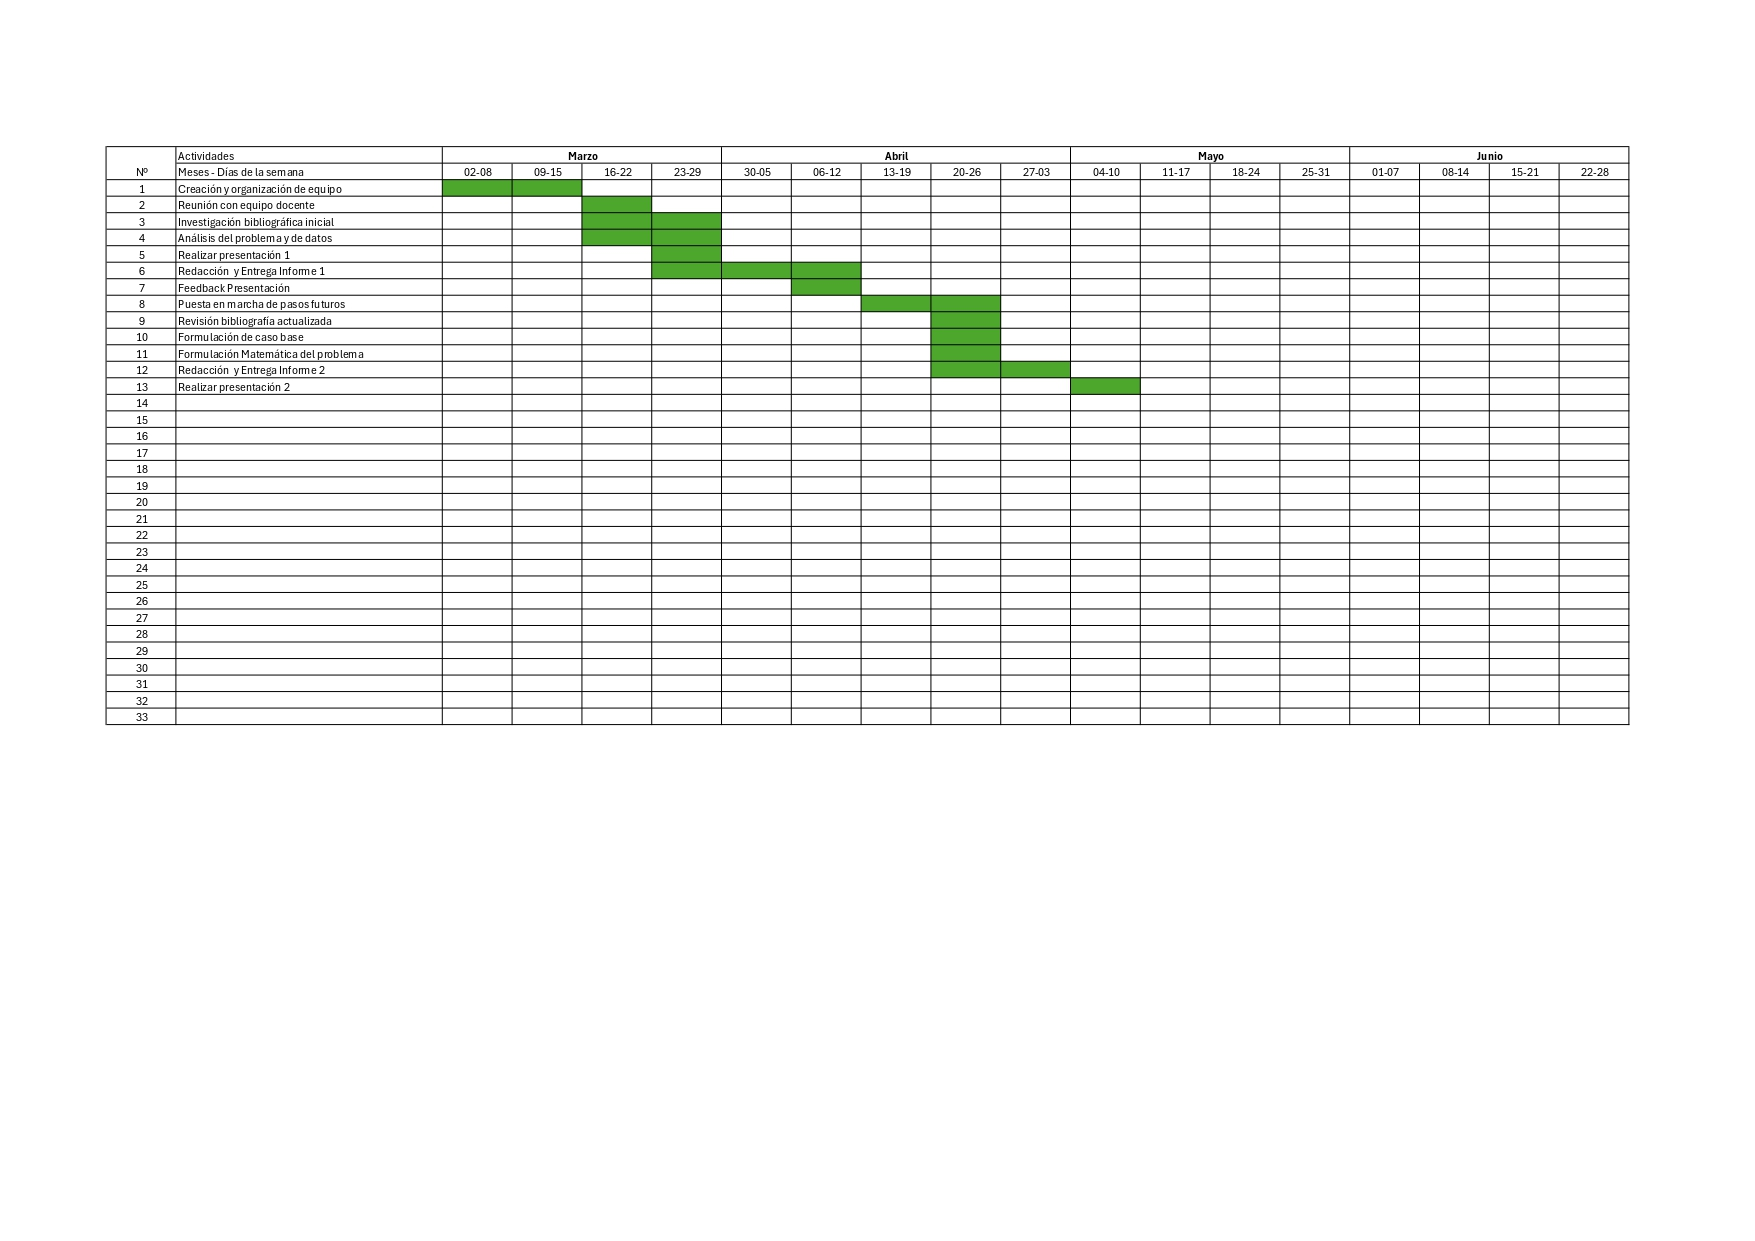
\includegraphics[width=1.2\textwidth, angle=90]{figures/Carta Gantt Capstone (1)_page-0001.jpg}
    \caption{Carta Gantt, Período Marzo-Mayo}
\end{figure}




\end{document}